\documentclass[11pt,a4paper]{article}
\usepackage[hmargin=3cm, vmargin=3cm]{geometry}
\usepackage[hangul]{xetexko}
\usepackage{blindtext}
\usepackage{parskip}
\usepackage{graphicx}
\usepackage{hyperref}
\usepackage{ulem}
\usepackage{float}
%\setmainhangulfont{KoPubBatang_Pro}[
%  BoldFont=KoPubBatang_Pro Bold
%]
\setmainhangulfont{Noto Serif CJK KR}
\setsanshangulfont{Noto Sans CJK KR}[
%  CharRaise=0.2ex
]
\newcommand{\sub}[1]{\textsubscript{#1}}
\newcommand{\awquote}[1]{\quote{#1}}
\setlength{\parindent}{20pt}
\linespread{1.5}
\begin{document}
\title{2017 웹 개발 길잡이}
\author{김대현 <\url{https://medium.com/@hatemogi}>}
\date{2017년 8월}
\maketitle
\section{시작하기}

\dotemph{개}발을 \dotemph{알}지 \dotemph{못}하는 당신이 웹 개발을 시작한다면, 어디서부터 무얼 공부해야 할지라는 주제의 글입니다. 감히 누구도 편하게 얘기하기 어려운 주제입니다. 무능한 저 한 개인이 올바른 가이드를 제시해 드릴 수 없는 일입니다만, 무책임하게나마 감히 적어보겠습니다. 너무 신뢰하지 마시고 가벼이 읽어 주시고, 이렇게 생각하는 사람도 있구나 정도로 넘기시면 좋은 주제입니다.

\textsf{간혹 주변에서 본격 웹 개발자가 되고 싶다}거나, 아니면 어떤 필요에 따라 웹 개발이라는 분야에 도전해 보려는 분들이 계신데, 마땅히 추천해 드릴 자료나 가이드가 너무 부족하다는 생각이 들었습니다. 그도 그럴 것이, 아직 웹 개발이라는 분야가 빠르게 성장하고 있고, 어제는 촉망받던 기술이 오늘의 레거시가 되버리는 상황이 반복되고 있어서, 정작 전업 개발자들조차 따라가고 배우기 벅찬 상황입니다. 뭐 하나 배워 놓으면 금세 쓰레기 지식이 되고 마는 거죠. 게다가 뭐 하나의 한 분야의 같은 일을 하는 데도 다양한 기술과 방법이 숱하게 쏟아지면서 서로가 좋은 방법이라며 싸움에 가까운 토론을 벌이고 있어서 혼란스럽습니다.

이런 상황에, 누군가 새로이 웹 개발에 도전해서 무언가 간단하게나마 만들고 싶다는 생각이 있다 하더라도, 무언가를 공부하고 있으면, 다른 누군가가 나타나서, 그게 아니라 이 방법이나 이 기술을 써야 한다며 훈수를 두는데, 잘 모르는 입장에서는 팔랑귀가 펄럭여서 새로 처음부터 시작하게 되기도 합니다.

맞습니다. 더 새로운 기술과 더 나은 도구들이 분명히 있습니다. 그런데, 개발자마다 성향과 상황과 또 그들의 과거 경험에 따른 선호도가 너무도 다르고 다양해서, 잘 정리된 가이드가 나오기는 힘들어 보입니다. 지금도 없었고, 앞으로도 없을 것입니다. 이 글 역시 그런 충분한 가이드일 수는 없습니다.

상황이 이러니, 이런 방법으로 도전해 보면 어떨까요? 우선 무언가 직접 만들어서 개발한 웹서비스를 온라인에 공개해 보는 겁니다. 아무도 안 쓰더라도 상관없습니다. 나 혼자 들어가 보고, 친구들에게 링크를 보내줍시다. 들어와 보고 ``이게 뭐냐?''라고 의아해하며 그냥 나가더라도 상관없습니다. 한번 만들어나 봅시다. 우아하고 최신의 기술이 아니어도 괜찮습니다. 일단 무언가 보이게 해 봅시다.

\section{목표}
이 글의 목표는 공부해야 할 주제와 키워드를 제시하는 것입니다. 그 상세 내용은 직접 찾아보며 하셔야겠지만, 전체 적인 계획과 꾸준한 노력을 투자할 기준점을 하나 세워드리는 것이 목표입니다. 취직이나 훌륭한 개발자가 되는 것이 목표도 아닙니다. 단지 내가 공부해서 웹서비스 하나 만들어 보는 것이 목표입니다. 안 그래도 어려운 개발, 생소한 개발, 목표를 간단하게 잡아 봅시다. 거창한 대규모의 웹서비스 아닙니다. 끽해야 백 명 쓸까 말까 한 서비스, 간단한 서비스입니다.

미리 말씀드리자면, 아무리 최대한 간단하고 얕게만 파고들더라도 긴 시간이 필요합니다. 일 투자 시간에 따라 다르겠지만, 수개월에서 수년이 넘게 걸릴 수도 있습니다. 이 글의 내용을 다 배우더라도 투자하는 노력에 비해 당장 눈에 보이는 결과가 보잘것없을 겁니다. 그럼에도 불구하고 시작해보겠다는 의지가 있으시다면 계속 읽어주시기 바랍니다.

\section{제공하는 가치}
개발 전체 과정에 있어 필요한 주제를 최소한 한 가지씩 꼽아드리겠습니다. 많아 봐야 두세 가지 중 하나를 택하면 되게끔 알려드리겠습니다. 접근하지 말아야 할 주제도 적어드리겠습니다. 시간을 낭비하는 함정에 빠질 일을 막아드리겠습니다. 당신이 뛰어야 할 젊은 말이라면, 양 눈 옆에 가리개를 가려드리겠습니다. 앞만 보고 뛰세요. 최단코스를 찾는라 고민하지 마세요. 우리의 목표는 갈팡질팡하지 않고 목적지를 향해 가는 겁니다, 조금 돌아가더라도요.

\section{제공하지 \dotemph{않는} 가치}
각 세세한 내용의 설명은 드리지 않습니다. 직접 해당 키워드로 찾아보시고 공부하셔야 합니다. 대부분의 내용은 이고잉님의 오픈튜토리얼스를 참고하시면 좋은 자료가 많을 것으로 생각합니다.

각 분야의 최고의 선택을 제시하지도 않습니다. 그저 되는 것 중에서, 제 개인이 선호하는 방법을 알려드립니다. 다른 개발자와의 의견은 얼마든지 다를 수 있습니다. 선택의 폭을 좁히는 것이 목표이지 최고 효율의 방법을 알려드리는 것이 목표는 아닙니다. 미리 귀뜀하자면, 이게 최선의 방법이다라고 주장하는 사람의 말을 듣지 마시라는 겁니다. 거짓말장이이거나 아직 무지한 사람일 가능성이 높습니다. 왜냐하면 이 바닥에서 최선의 방법을 제시하기는 꽤 어렵거든요.

\section{공부해야 할 주제}
정해진 카테고리는 아닙니다만, 대략 이렇게 나눠서 공략해 봅시다. 배우다 보면 한 주제에 대해서도 다양한 방법들이 즐비합니다.  언젠가 더 진지해진다면 더 깊게 다뤄야 하겠지만, 지금은 한눈팔지 말고 아주 얕게만 파기로 합니다. 누가 뭐라고 해도, 여기 정리한 선택만 하고, 나머지 선택은 외면해 버립시다. 이 주제들을 다 훑고 나면, 그 후에 누가 좋다고 한 기술을 더 알아보기로 합시다.

\begin{description}
\item[프론트엔드\sub{front-end}] 이용자의 웹브라우저에서 직접적으로 보이는 부분
\item[백엔드\sub{back-end}] 웹브라우저가 활용할 데이터를 관리하는 뒷단 일을 처리
\item[데이터베이스\sub{database}] 백엔드가 다루는 데이터를 보관하고 검색
\item[네트워크\sub{network}] 각 컴퓨터 사이의 데이터 통신
\item[에디터/툴/VCS\sub{tools}] 개발 작업에 필요한 도구의 선택과 활용
\item[기초 자료 구조\sub{data structure}] 데이터를 효과적으로 다루기 위한 기술
\item[리눅스/도커/AWS] 백엔드와 데이터베이스를 운영할 기술과 환경
\end{description}

아직 이 주제들이 무얼 의미하는지 몰라도 됩니다. 오늘 글에서는 이 주제들이 무얼 의미하고 어떤 걸 키워드로 전해드릴 지만 적어보겠습니다.

\section{프론트엔드}
흔히 \textsf{HTML, CSS, 자바스크립트\sub{JavaScript}} 등의 단어를 들어보셨다면, 이 주제가 그 영역을 의미한다고 보시면 됩니다. 우리가 사용하는 웹브라우저가 이해하는 직접적인 기술들을 다루는 분야입니다. 인터넷 익스플로러, 사파리, 크롬 등의 웹브라우저는 인터넷에서 문서를 받아와서 화면에 보이는데, 이 보이는 문서의 내용들이 들어있는 모양새라고 보시면 어떨까 합니다.

다른 거 빼고, \textsf{HTML5, CSS3, JavaScript}를 보시면 됩니다. 서툴지만 쉽게 얘기하면, \textsf{HTML5}는 웹문서 본문을 적는 텍스트 포맷이고, \textsf{CSS3}는 그 문서의 스타일을 다루는 속성들이며, \textsf{자바스크립트}는 웹브라우저가 이해하고 실행할 수 있는 프로그래밍 언어입니다. \textsf{HTML5}와 \textsf{CSS3}는 평범히 적는 텍스트지만, \textsf{자바스크립트}는 좀 더 본격적인 프로그래밍을 해야 합니다.

프론트엔드 기술만 다뤄도 내 컴퓨터에 저장한 파일로 웹브라우저 화면에 무언가를 보이게는 할 수 있습니다.

보통 프론트엔드에서 무언가 주문(요청)을 하고, 그 주문을 멀리서 받은 서버가 응답을 주고, 그 응답 내용을 웹브라우저가 화면에 표시합니다. 프론트엔드가 먼저 요청을 해서 서비스를 받는 입장이고, 백엔드가 그 요청을 받아서 작업을 처리하고 응답을 주는 입장이라서 각각 클라이언트 측\sub{Client-side}과 서버 측\sub{Server-side}라고도 부릅니다. 식당에 가면 손님(클라이언트)이 주문을 하고 웨이터나 웨이트리스(서버)가 주문을 받아서 주방에 전달해 요리를 만들어 다시 손님에게 가져다 주는 상황과 비슷합니다.

이 기본 기술을 편하게 잘 다루기 위해, \textsf{React.js / AngularJS / Vue.js} 등의 다양한 추가 요소들이 있습니다. 우선은 거들떠보지도 말고, 오로지 \textsf{HTML5, CSS3, \dotemph{기본} JavaScript}만 봅니다. 자바스크립트를 다루는 데에도 그 앞에 \textsf{TypeScript}를 쓴다거나 더 효과적인 도구나 언어들이 있습니다만, 역시 우선은 빠져들지 많습니다. 그냥 날것의 자바스크립트만 봅니다.

특히 프론트엔드는 엎치락 뒤치락 새로운 기술들이 하루가 다르게 뒤엎는 분야입니다. 각별히 주의합니다.

아직 언급할 단계는 아니지만, 이 연재의 컨셉을 미리 밝히는 의미로 말씀드리면, 이런식이 될 것 같습니다.

프론트엔드에서 처리하는 내용이 더 방대해지고, 웹서비스의 수준이 올라가면서, 이용자의 기대치도 높아졌기 때문에, 위 기본 세 기술을 그대로 써서 원하는 결과물을 만들기는 어려움이 많습니다. 그래서 저 3가지 기술요소들을 더 유연하고 멋지고 편하게 다루기 위해 아래의 기술들이 쓰이는 상황입니다.

\begin{itemize}
\item 보통의 웹사이트 처럼 간단한 화면 요소들만 필요할 것 같다면 \href{https://vuejs.org}{Vue.js}를 공부해서 쓰세요.
\item 흔히 보는 웹사이트들 보다 우아하고 현란하게 바뀔 내용이 많은 경우에는 \href{https://facebook.github.io/react}{React.js}를 공부해서 쓰세요.
\item \href{https://angularjs.org}{AngularJS}는 시작도 하지 마세요. 덩치 큰 괴물입니다.
\end{itemize}

이런 컨셉이라서, 분명 \textsf{AngularJS}를 선호하시는 분들은 싫어하실 겁니다. 앞으로도 아마도 본인이 싫어하는 내용이 보이면, 이 시리즈 전체를 폄하하시거나 공격적인 의견을 피력하실 수도 있습니다. 이해합니다. 저라도 그렇습니다.

이 글의 목표는 \textsf{Vue.js / React.js / AngularJS} 같은 어려운 주제들을 고르는 노력조차 줄이는 데 있습니다. 그걸 고르고 평가하고 선택하는데도 굉장한 에너지가 듭니다. 혹자는 또 이렇게 얘기할 겁니다. 저 셋을 동일 선상에 놓는 것도 이상하다고, 정확한 의미를 규정하려 하며 태클을 걸 것입니다. 그분들의 말이 정확하고 맞습니다. 하지만 이 연재에서 저는 정확성을 포기하고 크로키로 전체 흐름만을 잡도록 하겠습니다.

\section{백엔드}

백엔드는 프론트엔드에 보일 자료들을 만들어 내는 영역입니다. 자바, 파이썬, 루비 등의 언어나 스프링, 장고, 루비 온 레일스 같은 프레임워크 이름을 들어보셨다면, 그게 바로 이 영역입니다.

백엔드에서는 프론트엔드에 보여줄 HTML 문서를 그때그때 생성해서 내려줍니다. 한번 작성하고 잘 바뀌지 않는 내용들은 평범한 파일의 형태로 디스크에 저장해뒀다가 전달해주고, 그때그때 변하는 새로운 자료들은 요청시 클라이언트마다 다르게 만들어서 내려주고는 합니다. 전자를 정적\sub{static} 페이지라고 하고, 후자를 동적\sub{dynamic} 페이지라고 합니다. 모든 고객이 같은 걸 보는 메뉴판 같은 것을 정적\sub{static} 자원이라고 보면 되고, 고객마다 다른 응대를 해주는 웨이터/웨이트리스의 응대 기술이 동적\sub{dynamic} 영역이라고 보시면 될 것 같습니다.

백엔드는 여러 고객의 요청을 한꺼번에 받아서 각각 제대로 처리해서 내려줘야 하는 동시성\sub{concurrency} 처리 문제가 있어서 어려운 면이 있습니다. 요리 주문을 받은 주방에서는 요리사들이 다양한 재료를 한꺼번에 조리하면서 여러 요리가 각각 하나의 요리로 완성돼야 하는 상황과 비슷합니다. 요리사가 스테이크 요리를 하고 있는데, 스파게티 주문이 들어왔다고 해서 스테이크 요리에 토마토소스를 얹으면 안 되잖아요? 그렇다고 스테이크 요리가 끝날 때까지 기다렸다가 스파게티 요리를 시작하면 고객들은 이미 화를 내며 집에 갈 테고요. 그러니 여러 가스레인지에 여러 요리가 마구 동시에 조리돼야 하는데 이렇게 동시에 여러 작업을 하면서도 각각의 처리 단위가 서로 꼬이지 않게 완성되게 하는 일이 동시성 처리입니다. 동시성 처리를 잘 하면서, 성능까지 좋아야 많은 고객의 다룰 수 있기 때문에 다양하고 어려운 기술들이 많이 있습니다만, 우리의 목표는 대용량 서비스가 아닙니다. 간단한 서비스이므로, 동시성 처리를 문제없이 다루되, 빼어난 성능을 위한 기술들은 외면하도록 합시다. 동네 맛집을 운영할 거지 특급호텔 뷔페 주방을 운영할 게 아니거든요.

백엔드는 특히 성능 튜닝의 작업이 효과적으로 드러나는 분야라, 아주 사소한 영역까지 더 빠르게 개발하려는 노력이 깃드는 분야입니다만, 지금은 불필요한 잡기로 여기고 거들떠보지도 말도록 합니다.

백엔드는 특성상 프로그래밍 언어의 선택이 자유롭고 다양합니다. 앞서 언급한 대로 흔히 \textsf{Java, Python, Ruby} 등이 흔히 선택되고,  프론트엔드의 자바스크립트 언어를 백엔드에서 쓰는 \textsf{Node.js}도 있고, \textsf{Go}나 \textsf{Swift} 같은 언어도 있습니다. 제가 즐겁게 배우고 있는 \textsf{Clojure}도 쓸 수 있습니다만, 우선은 \textsf{Python}이나 \textsf{Ruby}중에서 고릅니다. 둘 다 가볍고 빠르게 더 많은 결과물을 만들어 낼 수 있습니다. 주변에서 \textsf{Java}를 권하는 사람들이 있을 텐데, 고맙다 말하고 무시하세요.

\textsf{Python}과 \textsf{Ruby} 프로그래밍 튜토리얼 사이트를 빠르게 훑어보시고, 조금이라도 더 끌리는 쪽으로 선택해서 백엔드 개발에 활용하시면 됩니다. 저 개인적으로는 \textsf{파이썬}이나 \textsf{루비}나 비슷해 보이고, 둘 중에는 \textsf{루비}를 선호합니다만, 적어도 국내 상황에서는 \textsf{루비}는 다소 식어있고, \textsf{파이썬}은 꽤나 흥하고 있습니다. \textsf{파이썬}의 경우 매년 열리는 컨퍼런스의 규모나 참석자 수를 보더라도 흥하고 있는 것을 알 수 있습니다. 다만, 웹 개발에는 \textsf{루비 온 레일스}라는 극강의 프레임워크가 \textsf{루비} 쪽에 있기 때문에, 딱 둘 중에 뭐다 우세를 정하기 어렵습니다. 국내 커뮤니티 규모의 측면에서는 \textsf{파이썬}, 웹개발의 편리함 측면에서는 \textsf{루비}를 선택하면 되겠습니다. \textsf{파이썬}도 \textsf{장고} 같은 프레임워크가 잘 돼있기 때문에 아주 큰 차이는 아닐 겁니다.

다만, \textsf{Java}는 무시하도록 합니다. 우리가 짓고자 하는 것은 2층 목조 주택인데, 대형 아파트 단지를 지을 언어를 선택할 이유는 없습니다. 그리고, 프론트엔드 개발부터 시작하신 분들은 자바스크립트 언어를 써서 백엔드 개발을 하는 \textsf{Node.js}를 선택하기도 합니다. 나쁘지 않습니다만 일단 제외합니다. 쉽게 접근할 수 있는 \textsf{PHP}를 권하는 사람도 있을 겁니다. 고맙다 말하고 무시하세요.

\begin{itemize}
\item \emph{Do} -  루비나 파이썬 중에 고르세요.
\item \emph{Don't} - 자바나 PHP는 거들떠보지도 마세요.
\end{itemize}

\subsection{흘러가는 기술들}

이 글의 방향성을 밝히고자, 조금 미리 \textsf{React나 Vue.js} 같은 주제를 말씀드렸습니다만, 다시 강조하자면, 그런 주제를 시작하기에 앞서서 \textsf{HTML5, CSS3, Javascript} 기초를 먼저 닦아두는 편이 좋습니다. 흔히 우리는 무언가 공부해야 하는 주제가 쌓여있을 때, 조급한 마음에 기초를 건너뛰고 지금 당장 쓰이는 기술에 먼저 접근하려는 유혹에 빠지는데, 그래 봤자 다시 기초로 돌아와야 해서 오히려 더 느리게 나아가게 되기도 합니다. 유행하는 기술을 빨리 공부하고 싶은 조급한 마음은 잠시 가라앉히고, 기초부터 닦는 게 실질적 도움이 더 크기도 해요. 그리고, 어차피 \textsf{React나 Vue.js} 같은 것들은 2~3년이 지나면 또 언제 핫했냐는 듯 금세 유행이 가고 더 새로운 기술로 그 관심이 옮겨갑니다. 빠르게 변하는 분야는, 어제의 핫한 기술이 오늘의 폐품이 되는 주기가 굉장히 짧습니다.

그래서 기초를 잘 쌓으면서, 그 위에 유행하는 기술은 잘 익혀서 유통기한 내에 잘 써먹고 잊으면 됩니다. 핫한 기술들은 지식을 축적하는 게 아니라 소비하는 일이라고 보면 좋습니다. 잘 씹어 먹고 잘 소화해서 그 날의 에너지원으로 삼으면 됩니다. 굳이 그 지식들을 뼛속 깊이 쌓아둘 필요는 없어요. 너무 오래 쌓아두면 오히려 독소가 됩니다. 반면, 기초가 되는 기술들은 뼈로 만들기까지 시간이 좀 들고, 당장은 쓸모없어 보이기도 합니다만, 일단 뼈가 되고 나면 그 위에 지방을 쌓든 근육을 키우든, 중요한 버팀목이 되어줍니다. 뼈와 지방은, 어느 한쪽이 중요하고 다른 쪽이 덜 중요한 것이 아니라, 성격과 활용이 다른 것뿐이고 둘 다 중요하고 필요합니다. 다만 보통 초심자들이 겉에 잘 드러나는 지방과 근육에 쉽게 현혹되기 때문에, 이 연재에서는 균형을 맞추고자 뼈를 만드는 쪽을 좀 더 강조하는 입장을 취하도록 하겠습니다.

다시 말해 \textsf{React나 Vue.js}는 요새의 \emph{칼로리원이나 근육으로 삼으면} 되고, \textsf{HTML5, CSS3, Javascript}로는 \emph{탄탄한 뼈를 만들면} 됩니다. 뼈가 없으면 애써 근육을 만들어봐야 지지대가 없어서 힘을 쓸 수 없겠죠? 한편, 우리 몸의 뼈도 보통 6개월이 지나면 완전히 새로운 세포로 교체된다고 하더군요. 기초 기술이라고 해서 영원한 것은 아니고, 단지 지방이나 근육보다 조금 더 오래가는 것뿐이에요.

자, 그럼 이제 모호한 얘기는 이쯤에서 줄이고, 이어서 이번 편에는 ``데이터베이스''와 ``네트워크''에 대해 어디서부터 공부하면 좋을지 정리해볼게요.

\section[database]{데이터베이스\sub{database}}

드디어 우리 웹서비스의 데이터를 저장할 방법을 알아볼 때입니다. 보통 프론트엔드와 백엔드는 오가는 데이터를 처리하면서 일시적인 부분만을 잠깐씩 기억하면서 활용하며, 실제로 오래 보관할 내용은 데이터베이스에 기록합니다.

데이터베이스의 사전적 의미는 ``잘 정돈한 데이터의 모음''입니다. 우리가 필요한 데이터를 잘 기록하면서, 필요한 때에 찾아보기 좋게 잘 정돈해 놓는 거지요. 흔히 약자로 DB라고 부르는데, 데이터 모음을 포함해서, 그 데이터 모음을 관리하는 시스템이나 소프트웨어를 뭉뚱그려 부르기도 합니다. (정확하게 말하자면, 후자는 DBMS라고 구분해서 말해야 하는데 그러지 않아도 널리 이해하는 분위기인 것 같습니다.)

DB도 종류가 여럿인데, 가장 널리 쓰이는 것은 RDB라고 관계형(Relational) 데이터베이스입니다.  MySQL, PostgreSQL, Oracle 등이 RDB이지요. 대부분 RDB를 쓰기에 DB라고만 해도 RDB를 뜻하기도 합니다.

DB에 컬럼, 레코드, 테이블의 구조를 갖춰 데이터를 기록하는데, 이는 우리가 흔히 쓰는 스프레드시트 프로그램의 구조와 비슷합니다. 엑셀이나 구글시트의 시트가 DB의 테이블이고, 각 시트의 행이 레코드이며, 열이 컬럼입니다. 엑셀로 가계부를 정리할 때, 날짜/내역/금액/비고 등의 열을 두고, 각각의 행에 입출금 내역을 적어 놓는 것과 같습니다.

\begin{tabular}{|ccc|}
  \hline
  가계부(시트) & $\Leftrightarrow$ & 테이블  \\
  날짝/내역/금액/비고(열) & $\Leftrightarrow$ & 컬럼 \\
  일출금 내역(행) & $\Leftrightarrow$ & 레코드 \\
  \hline
\end{tabular}

영수증을 어딘가에 잘 쌓아두기만 해도 될 텐데, 왜 굳이 엑셀에 힘들게 적어 놓나요? 기초 자료를 바탕으로 잔액이나 총 지출/수입 등을 자동으로 계산할 수 있고, 특정 날짜의 항목을 찾거나, 내역의 텍스트나 금액을 기준으로 검색해서 찾아보기 쉽기 때문 아닌가요? 기록으로 보관하려는 의도도 있고, 계산과 검색이 편한 구조로 남겨두는 목적도 있습니다.

엑셀 등에 담는 시트가 테이블인 셈인데, 관계형 데이터베이스는 그 안의 여러 테이블 사이에 관계를 다루는 연산들이 있습니다. 한 테이블만을 대상으로 해서 계산하거나 검색하는 범위를 넘어서, 두 테이블 이상을 합쳐서 무언가 계산하거나 검색하는 경우도 많습니다.

DB에 연산을 요청하는 내용을 쿼리\sub{query}라고 부릅니다. 우리말로 `질의'라고 번역하거나 그냥 쿼리라고 부릅니다. 이 쿼리는 꽤 유연하고 강력한 기능들이 많이 필요하기에, 하나의 언어로 되어있습니다. 이 언어의 표준 격으로  SQL\sub{Structuered Query Language}, 구조화된 질의 언어)이라는 것이 있고, 각 DB 제품마다 조금씩 다른 방언\sub{dialect}을 씁니다. 서울말을 바탕으로 한 표준어가 있고, 각 지방에서 쓰이는 방언들이 조금씩 다르지만 대개는 의사소통이 되는 것 상황과 비슷합니다. MySQL에서 쓰는 쿼리와, PostgreSQL에서 쓰는 쿼리가 거의 비슷하면서도 세세한 부분이 조금씩 다릅니다.

휴, 여기까지만 해도, 앱 개발을 위해 자바스크립트, (루비 or 파이썬), SQL까지 세 개의 복잡해 보이는 언어를 배워야 하게 되었네요. HTML도 사실상 마크업 \dotemph{언어}이기 때문에 그런 것까지 언어라고 말하면 금세 더 배워야 할 언어의 수가 늘어납니다. 하지만, 언어라고 해서 너무 겁먹을 필요는 없습니다. 영어나 중국어를 배우는 것처럼 어려운 일은 아닙니다. 문서도 잘 돼있고, 보통 좋은 언어들은 그 표현 자체가 단순하며, 무엇보다 쓰는 순간마다 도와주는 도구가 아주 잘 돼 있어서, 대충 얘기해도 철석같이 잘 알아들을 수 있는 표현으로 바꿔주며, 조금이라도 틀린 표현이 나오면 자동으로 알려줍니다. 내가 콩글리시로 대충 얘기해도 늘 따라다니는 미국인이 그 자리에서 정확한 표현으로 통역해주는 상황이랄까요? 다만, 너무 어긋나면 통역이 불가능하겠지만요.

아무튼, 이쯤에서 DB도 제품을 골라야 하겠습니다. 지금 상황에서는 MySQL이 가장 널리 쓰이는 것 같습니다. 책도 많이 나와있고요. 다만 저 개인적으로는 MySQL이 오라클에 인수됐기 때문에 능동적으로 발전해 나가야 할 이유가 줄어들었다고 생각합니다. 아마 그 흐름을 MariaDB가 이어받는게 아닌가 합니다만, 그냥 전 속 편하게 PostgreSQL을 쓰자는 입장이기에 잘 모르겠습니다. 안전한 선택을 하시려면 MySQL, 그 보다는 마이너하지만 제대로 된 선택을 하시려면 PostgreSQL을 택하시면 되겠습니다. 그렇다고 MySQL이 제대로 된 것이 아니라는 뜻은 아닙니다. 아 참 이거 조심스럽네요. 매번 말씀드리듯, 적지 않은 기술적 선택에 개인 취향이 많이 작용합니다. 정리하자면, MySQL이나 PostgreSQL 중에 고르면 됩니다. 이 역시 주변에서 Oracle이나 Microsoft SQL Server 등을 권하기도 할 겁니다. 고맙다 말하고 무시합니다. 마침 서울에 출장 온 김에 대형 서점에 들러서 둘러 보았더니, 역시나 오라클과 SQL Server 책이 많더군요. 아무래도 기업들이 많이 쓰는 제품이라 그런 것 같습니다. 우리는 기존 기업에 취직해서 DBA가 될 게 아니라, 내가 원하는 작은 웹서비스를 만들 것이므로 깔끔히 외면하도록 합니다. 그래도 MariaDB나 MySQL 책은 더러 있었는데, 아쉽게도 PostgreSQL책은 레퍼런스 사이트를 번역한 책 한 권 밖에 찾지 못했습니다. 그래서 PostgreSQL로 선택하신다면, SQL 기본 서적을 보면서 공식 웹사이트 매뉴얼을 참고하시는 방법이 좋을 것 같습니다.

한편, DB는 데이터를 보관한다는 측면에서 워낙 중요하고, 또 오랜 기간 중요하게 기능하며 발전해 왔기에, 이용하는 입장에서도 어렵지만, 그걸 관리하고 운영하는 입장은 훨씬 더 어려운 면이 있습니다. 데이터를 잘 남겨두고, 주기적으로 백업(별도 보관)하고 혹시라도 장애가 나면 복구해야 하며, 때로는 데이터를 다른 곳으로 옮겨야 하며, 새로 구축해야 할 때도 있습니다.  관리\sub{Administration}의 측면만 봐도 큰 일이고 전문적이어서 그 직종이 따로 있고, 큰 회사들은 전담 팀과 부서가 따로 있는 경우가 많습니다. 그러나 역시 겁먹을 필요는 없습니다. 2층 집을 짓는 우리에게는 별도 인력을 확보할 여력이 없기도 하고, 다행히도, 앞으로 사용할 AWS 같은 환경에서는 그 관리의 행위와 역할이 클라우드 쪽으로 대폭 옮겨 가서, 개발자가 직접 해야 할 일이 훨씬 줄었습니다. 백업이나 복구 같은 일만 해도 꽤 어렵고 힘든 일인데, 요새는 AWS 콘솔에서 클릭 몇 번 하면 알아서 잘 해주지요. 아직 설명하지 않은 시스템 운영 측면에서도, 이 시대의 인프라 시스템이 너무 잘 돼 있어서, 사실 그 어느 때보다도 한 개인이 완전한 서비스를 만들어 내기 쉬운 환경이 됐습니다. 앞으로 더 쉬워지겠지요.

다시 데이터베이스의 이용 측면으로 돌아와서, 웹 개발자 입장에서는 우리가 고른 루비나 파이썬 백엔드 프로그램에서 데이터베이스에 접근해서 새 데이터를 기록하거나, 이미 기록한 데이터를 잘 조회해서 보여주는 일을 합니다. 그때 우리가 만드는 백엔드 소프트웨어(웹서비스)가 DB와 통신하기 위해 사용하는 언어가 SQL입니다. 백엔드가 직접 SQL을 거의 그대로 쓰는 경우는 요새는 별로 없고, 그 사이에 조금 더 편리한 계층이 있습니다. 루비온레일스의 경우에는 액티브레코드\sub{ActiveRecord}라는 라이브러리가 그 일을 합니다. DB서버가 다루는 집합(set) 구조의 레코드와 컬럼을 객채지향 프로그램에서 다루기 좋은 형태로 변환하는 일을 하지요. 이 형태가 아직 통일된 것은 아니라, 각 언어별로 조금씩 다른 구조를 취하기도 합니다. 예를 들어 자바에서는 JPA라는 표준이 있어서 그런 일을 담당합니다. 루비온레일스의 액티브레코드 같은 경우는, 적어도 제가 써 본 것들 중에는 가장 우아하고 강력한 기능을 자랑했습니다. 아무래도 이질적인 무언가를 매개하는 일을 할 때는 보다 유연한 언어가 유리한 것 같습니다.

액티브레코드처럼 훌륭한 지원 도구가 있는 경우에는 SQL을 아주 기본적으로만 알아도 됩니다. 복잡한 구문들을 액티브레코드가 대신 처리해주니까 말이죠. 하지만, 그렇다고 SQL을 몰라도 된다는 뜻은 아닙니다. 복잡하고 번거로운 작업을 아주 편리하게 대신해주는 겁니다.

그래서 DB를 하나 골라서, SQL의 기초를 공부해가며 테이블과 관계를 다루는 법을 익히면서, 우리가 택한 언어에서 널리 쓰이는 DB 접근 레이어를 써서 유연하게 데이터를 다룰 수 있게끔 공부하면 되겠습니다.

\begin{itemize}
\item \emph{DO} - MySQL or PostgreSQL
\item \emph{DON'T} - Oracle nor SQL Server
\end{itemize}

완전히 다른 얘기로, 데이터베이스라는 것이 결국, 우리가 만드는 웹서비스에 잘 정리하고 나중에 찾아볼 데이터를 잘 다룰 수 있으면 되는 겁니다. 그 형태가 꼭 관계형 DB일 필요는 없지요. 만약 그냥 디스크에 파일로 저장하거나 엘라스틱 서치 같은 검색 엔진에 부어 넣고도 내가 원하는 기능을 만들 수 있다면 그렇게 쓰면 됩니다. 그래서 RDB 말고도 MongoDB나 AWS의 DynamoDB를 비롯해서 다양한 형태의 데이터베이스가 널리 쓰이고 있습니다. 어쩌면 사람들이 너무 RDB에 치우쳐 있기에, 경우에 따라 다른 방식의 접근이 더 좋은 경우도 있다는 것을 잊게 되기도 하는 것 같습니다. 그리고 RDB를 쓴다고 해서 반드시 100\% 모든 데이터를 RDB에 담아야 하는 것도 아닙니다. 대부분은 RDB에 담고, 경우에 따라서 다른 형태로 저장해도 되지요. 그러니 RDB를 공부한다고 해서, 세상의 데이터베이스가 RDB가 전부다라는 생각으로 굳어지지는 말아야 하겠습니다. 분명, RDB는 오랜 기간 발전하면서 매우 성숙한 제품과 기술들이 함께 진보했기 때문에 가장 안전한 선택입니다만 말이죠.

한 가지 더, 한 귀로 흘려들으실 여담으로, 제가 만약 RDB 외에 선택 다른(?) DB를 쓴다면 Datomic이라는 제품을 쓰겠습니다. 아직 널리 알려지지 않았고, 상용 제품이기에 접근성이 떨어집니다만, 불변\sub{immutable} 데이터베이스라는 점이 아주 매력적으로 보입니다. 아직은 좀 기다려 봐야죠. 발상과 접근이 너무 좋아서, 곧 비슷한 접근 방식을 취하는 오픈소스 제품이 나와서 함께 발전하지 않을까 생각하고 있습니다. 그리고 조금 더 용기가 난다면, 돈을 내고라도 써 볼 만한 제품이라고 눈독 들이고 있습니다. 유료라고 해서, 오라클 같은 대기업용 제품처럼 막대한 비용이 필요한 건 아니니까요. 아니면, AWS위에서 과금제로 쓰는 만큼 돈을 내는 Datomic이 출시될 수도 있으니, 그걸 써도 괜찮지 않을까 합니다.

괜한 딴 얘기를 했네요. 우선 RDB 하나 골라서 공부하며 씁시다! RDB의 단점으로 지적되는 부분들이, 적어도 우리가 목표로 하는 동네 웹서비스 영역에서는 문제점으로 드러날 일은 없다고 생각해요. 나중에 AWS를 언급하면서 RDS 서비스를 말씀 드릴 텐데, MySQL, PostgreSQL 다 편하게 쓸 수 있으니, 고르시기만 하면 됩니다. \emph{거 참 좋은 세상!}

\begin{quote}
  \emph{요약} - MySQL이나 PostgreSQL을 고르고, SQL을 공부해 가며, 내가 택한 언어의 DB 접근 라이브러리를 써서 연습한다.
\end{quote}

\section{네트워크}
네트워크야 익숙하시죠? 우리 어디 가서 WiFi 안되면 공황상태에 빠지잖아요? 너무 익숙해서 모른다고 말하기 민망할 지경이죠. 우리 장비들이 서로 통신하는 망을 네트워크라고 합니다. 오래전에는 다른 네트워크 방식이 많았지만, (지금도 은행같은 금융권이야 다른 망을 많이 쓰겠지만) 요새야 네트워크라고 하면 인터넷을 의미하는 거죠. 간단하게만 얘기하자면, 우리가 쓰는 컴퓨터와 저 멀리 있는 백엔드 서버와 통신하는 연결선이라고 생각하면 어떨까 합니다.

어떤 장비가 네트워크에 연결되면, 고유의 주소를 할당받습니다. IP라고 줄여 부르는 이 주소가 인터넷에서의 주소입니다.  Internet Protocol 주소의 약자인데, 인터넷에서 쓰는 주소라고 생각하시면 되겠습니다. 모든 장비에 이 IP주소가 있어야 서로 통신이 됩니다. 내가 편지를 어디론가 보내려면, 받는 사람 주소가 있어야 하는 것처럼 당연한 일입니다. 생긴 모습은,

\begin{awquote}
104.74.171.196
\end{awquote}

이렇게 네 뭉치 숫자가 마침표로 이어진 모양으로 생겼습니다. 각 숫자가 1바이트라서 최대 255까지 표현합니다. 숫자상으로는 `0.0.0.0'부터 `255.255.255.255'까지 표현할 수 있습니다만, 중간중간 영역이 특별한 용도로 제외되기 때문에 모든 숫자를 다 쓰는 것은 아닙니다. 이렇게 4바이트로 인터넷 주소를 쓰는 것을 IPv4(Internet Protocol version 4) 주소라고 합니다. 특별한 목적으로 제외된 영역을 빼고 단순하게 계산해도 4바이트로는 $2^{32}$인 42억 개 정도를 쓸 수 없습니다. 이 주소를 IANA라는 단체에서 영역으로 떼어서 전세계 인터넷 서비스 제공업체에 할당해 주는데, 2011년 3월에 동이 났다고 하는군요. 실제로 전세계에서 42억 개 정도를 다 쓰는 것은 아니겠지만, 과잉 할당된 곳도 있을 테고, 또 워낙 세상에 장비들이 많으니 그럴 만도 합니다.

그래서 IPv6(Internet Protocol version 6) 주소를 쓰게 됩니다. 16바이트로 인터넷 세상의 주소를 표현하는 거지요. 16바이트로 표현하면 $2^{128}$ 개의 주소를 표현할 수 있으므로, 적어도 우리가 살아있는 동안에 부족할 일은 없어 보입니다.

\begin{figure}[H]
\centering
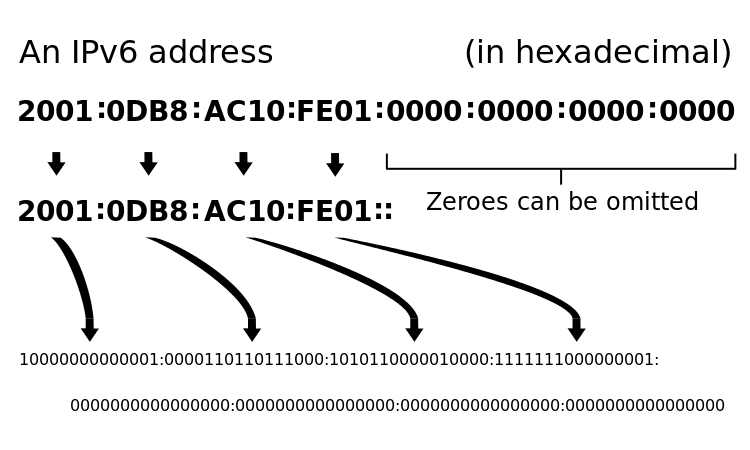
\includegraphics[width=\textwidth]{ipv6_address.png}
\caption{IPv6 주소 <\url{https://en.wikipedia.org/wiki/IPv6}>}
\end{figure}

이렇게 생겼다는데, 거 참 생소하네요.

요새야 거의 모든 장비와 서비스가 IPv4와 IPv6를 함께 지원하지만, 적어도 국내 환경에서는 그다지 호응이 없어 보입니다. 정확한 이유야 모르겠지만, 아마도 우리나라에 할당된 IPv4 주소 영역이 매우 넉넉하기 때문이 아닐까요? 부족하지 않으니 아쉬울 것이 없어서 우물을 팔 필요가 없는 거지요. 그래서 아직은 IPv4 만 알아도 되겠습니다만, 좀 익숙해지고 나서 IPv6도 신경 쓰면 좋겠지요.

IPv4건 IPv6건, 이 주소로 원하는 목적지에 요청을 보내야 하는데, 보시다시피 이 주소는 우리가 일일이 외우기는 어렵습니다. 네이버나 구글에 접속해서 검색을 해봐야 하는데, 저런 숫자로 접근해서 봐야 한다면 참 골치 아픈 일이 아니겠습니까?

그래서 전화번호부 역할을 해주는 서비스가 있습니다. 114 전화해서 ``네이버'' 얘기하면 ``네이버'' 전화번호를 알려주는 것처럼요. 그럼 우리는 여러 서비스의 전화번호를 외우지 않아도 됩니다. ``114''라는 전화번호 하나만 외우고 있으면 되지요. 그런 전화번호부 역할을 해주는 것이 DNS입니다. 도메인 이름 시스템\sub{Domain Name System}이라고, 우리가 읽을 수 있는 문자로 표현합니다.

\begin{quote}
www.naver.com
\end{quote}

이렇게요. 저 이름이 사실은 `104.74.171.196'를 대신하는 주소명인 겁니다. 저 주소명을 IP주소로 알아내는 작업을 DNS 조회\sub{look up}라고 합니다. 114에 전화 걸어서 상표명 묻는 행위인 거죠. 난 114를 입력한 적이 없는데 어떻게 그런 일을 하냐고요? 우리 장비가 인터넷에 연결되면, 우리 장비에 임시 IP주소를 할당해 주면서 DNS 서버 주소도 함께 줍니다. 그 114 역할을 하는 IP주소를 우리 컴퓨터나 스마트폰의 장비가 잘 기억하고, 그때그때 물어봐가며 IP 주소를 가져와서 원하는 목적지에 연결해 주는 작업을 합니다.

IP주소도 유한한 자원입니다만, 저 도메인명도 희소한 유한 자원이기에, 돈을 주고 삽니다. 1년에 돈 만원 정도 내면 해당 이름을 내가 원하는 IP주소에 연결하는 일을 해둘 수 있습니다. 자기 블로그 자기 도메인 명으로 운영하는 사람들 있죠? 그 도메인을 도메인 등록 서비스 업체에서 산 거에요. 우리도 돈 만원쯤 내서 사면 우리 백엔드 서버들에 할당된 IP주소로 쉽게 접근할 수 있도록 전화번호부\sub{DNS}에 등재해 둘 수 있습니다.

DNS를 거쳐서 알아내든, 직접 외우고 있었든 이제 IP주소를 알았습니다. 그다음 포트에 대해서 알아볼게요. IP주소는 보통 한 장비를 의미하고, 한 장비 내에서도 포트\sub{port}라는 것이 여러 개 있습니다. 포트는 2바이트로 0\textasciitilde65535 사이의 숫자를 씁니다.  0번과 49152번 이후의 숫자를 특별한 용도로 제외하고 그 사이의 숫자로 약 5만 개의 포트를 쓸 수 있습니다.

포트는, 반드시 그런 것은 아닙니다만, 각 통신 목적에 맞는 포트 번호 관례가 있습니다. 예를 들어 우리 웹브라우저로 접근하는 웹서비스의 경우 80번 포트를 써요. 암호화된 통신의 경우는 443번 포트를 쓰고요. 웹서비스 통신에 오고 가는 데이터 규약을 HTTP라고 부르는데, 이걸 암호화하지 않고 주고 받는 경우는 80번 포트로 접근하고, 암호화해서 주고 받는 경우에는 443번 포트에 접근합니다.

즉, 브라우저에서 아래처럼 치는 것은

\begin{quote}
http://www.naver.com/
\end{quote}

사실상

\begin{quote}
http://www.naver.com:80/
\end{quote}

과 동일합니다. 저런 주소 전체를 URL이라고 부르는데, 앞에 `http'가 프로토콜이고 `www.naver.com'이 도메인 명이며 `80'이 포트번호입니다. 암호화한 데이터를 주고받는 `https'의 경우는,

\begin{quote}
\quote{https://www.naver.com/}
\end{quote}

으로 접근하고, 이는 사실상

\begin{quote}
\quote{https://www.naver.com:443/}
\end{quote}

으로 접근한 것과 같습니다. 이 글을 쓰는 현재 http로 네이버에 접근하면, 자동으로 암호화된 https로 다시 연결하게 처리해주네요. 무조건 암호화된 통신을 하겠다는 얘기입니다.

우리가 웹서비스를 만들면 우선 80 포트 기준으로 백엔드 서비스를 띄워놓고 개발하다가, 나중에 도메인도 사고, 친구들에게 공개하기 전에는 폼나게 443번 포트에 암호화된 웹서비스를 올려두도록 합시다. 여기에는 TLS 인증서를 발급받아서 올려놓아야 하는데, 요새는 무료로 제공하는 서비스도 있기에 아주 어려운 일은 아닙니다. 혹시 연재가 길어진다면 그 부분도 적도록 할게요.

네트워크도, 조금 살펴보니 의외로 재밌지 않나요? 더 관심이 가신다면 네트워크 관련 서적을 더 살펴보시면 제 어설픈 설명보다 훨씬 잘 정리된 내용을 보시기 좋을 거예요.

그다음으로, 네트워크 기초를 보고 나면, 웹브라우저와 우리가 만들 백엔드 서버가 HTML, CSS, Javascript 파일 등을 주고받을 때 쓰는 프로토콜인 HTTP에 대해서도 살펴보도록 합시다. HTTP는 현재는 버전 1.1이 널리 쓰이고 있고, 2.0도 거의 모든 웹브라우저가 지원하며, 2017년 5월 기준, 상위 1천만 개의 웹사이트 중 13.7\%가 지원하고 있다고 나와있으나, 체감상 아직 널리 쓰이는 것 같지는 않습니다. 이 점도, 아쉬운 사람이 우물을 파야 하는데, 구글이나 네이버 같은 대형 서비스 제공업체에서나 엄청난 망 비용을 절약하고 싶어서 아쉬운 거지, 소규모 서비스 제공자 입장에서야 그다지 아쉬운 상황이 아니라서 말이죠. 그래도 언젠가는 2.0이 널리 쓰이겠지요. 아마도 IPv6가 안착할 때쯤? ㅎㅎ

이상 네트워크는, 제가 쉽게 설명하기에는 좀 무리가 있는 카테고리였음을 인정합니다. 솔직히, 뭐라고 요약해야 할지도 잘 모르겠네요.

\begin{verse}
요약: 인터넷 네트워크 기초 서적을 한 권 살펴보고, HTTP/1.1 프로토콜의 기초를 파악한다.
\end{verse}

\section{텍스트 에디터}

개발은 글쓰기와 상당히 유사합니다. 원고지에 글을 쓰든, 타자기로 쓰든, 워드프로세서로 쓰든 결국 텍스트를 적는 행위이고, 그 텍스트를 인쇄해서 책자로 만들어 독자에게 전달하는 것처럼, 개발자도 소스코드라고 부르는 프로그램 텍스트를 작성해서 그것을 프로그램으로 변환해서 배포하고, 그 프로그램을 이용하는 사용자가 쓰게 됩니다. 다소 다른 점이라면, 이용자들은 소스코드를 직접 보지는 않고 프로그램의 겉모습 만을 본다는 점 정도랄까요? 그래도 개발 과정에서는 함께 개발하는 멤버들이 서로의 텍스트를 함께 보고 같이 고쳐가며 개발하므로, 적어도 개발자들끼리는 그 소스코드를 함께 읽고 씁니다.

결국 이 텍스트는 대부분의 프로그래밍 언어가 알파벳, 숫자, 몇몇 특수문자를 활용해서 작성합니다. 대부분의 프로그래밍 언어가 텍스트에 유니코드를 허용하기 때문에 한글로 작성해도 괜찮은 경우가 많습니다만, 대부분의 프로그래머들은 영문자 위주로만 작성하는 것으로 보입니다(e.g. 한글코딩\footnote{\url{http://hangul-coding.org}}).

이 텍스트는 텍스트 에디터라는 프로그램으로 작성하고 편집할 수 있습니다. 70년대부터 쓰이던 텍스트 에디터인 Emacs\footnote{\url{https://www.gnu.org/software/emacs/}}와 Vim\footnote{\url{http://www.vim.org}}이라는 두 제품이 가장 강력하다고 정평이 나있고, 저도 이맥스를 쓰기는 합니다만, 몇 년을 써도 익숙하다고 얘기하기 어려운 면이 있습니다. 제 능력 부족이겠지요. 때로 이맥스교와 빔교의 교인들이 서로 종교 전쟁을 벌이는 경우도 볼 수 있고, 혹시나 주변 개발자가 이 종교(?)의 교인이라면 이런 에디터를 공부하라고 얘기하겠지만, 고맙다 얘기하고 무시합시다. 정말 강력한 것은 틀림없지만, 그냥 더 접근하기 쉬운 에디터를 써도 되지 않을까 하는 생각이 듭니다. 요새 가장 추천할 만한 에디터로는 Atom\footnote{\url{https://atom.io}}이 제일 좋지 않을까 합니다.

혹시 프론트엔드 개발만 집중해보겠다면 Brackets\footnote{\url{http://brackets.io}}도 꽤 편리해 보입니다.

예전에야 서버에 직접 접속해서 텍스트를 편집해야 할 일도 잦기 때문에 서버에서도 잘 실행하기 좋은 이맥스나 Vi가 유력했지만, 요새는 서버에 직접 접속해서 편집할 일은 점점 줄어드는 것 같습니다. 그냥 내 작업용 컴퓨터에서 실행해서 다루기 편리한 에디터를 골라 쓰도록 합니다.

\begin{itemize}
\item \emph{Do} - Atom
\item \emph{Don't} - Emacs, Vim
\end{itemize}

물론 세계 최강인 이맥스와 빔이 나쁘다는 뜻은 아닙니다. 익히면 정말 강력하고 멋진 기능은 기본에다가, 뭔가 제대로 된 실력자가 된 것 같은 포스도 덤으로 따라옵니다.  저도 ``난 이맥스 써'' 이렇게 한마디 말할 때에도 괜히 어깨에 힘이 들어가곤 하지요. 안 쓰는 사람들도, ``오 그래? (대단한 녀석이다)''라는 내색을 하기도 합니다. 이미 근 반 백 년 발전한 에디터이니 만큼, 앞으로도 오래 쓰이겠지요. 다만, 그렇게 강력하고 우아하게 쓸 수 있게 되기까지 너무 오랜 노력이 필요하다는 점이 좀 아쉽지요. Atom 같은 현대의 편리한 에디터가 더 발달하기를 기대해 보는 편도 좋을 것 같습니다. 이미 대부분의 활용면에서는 충분히 발달해 있습니다.

\section{통합 개발 환경}

Atom처럼 개발자를 위한 텍스트 에디터의 경우, 각종 개발자용 플러그인이 많이 나와있어서, 그대로 개발 작업에 써도 충분한 경우가 많습니다만, 때로는 전용의 통합 개발 환경 프로그램을 쓰는 것이 나은 경우도 있습니다. 예를 들어, Java 개발환경의 경우 인텔리J 라는 통합 개발 환경\sub{IDE}\footnote{Integrated Development Environment}에서 개발하는 것으로 결론이 난 상황으로 보입니다. 다양한 기능이 덧붙은 유료 버전도 있지만, 제가 업무용으로 사용하는 수준에서도 무료 버전으로도 충분합니다.

텍스트 에디터를 내포하고, 그 외에도 실행, 테스트, 디버그, 빌드 등의 다양한 개발 작업을 하나의 통합된 툴에서 개발할 수 있습니다. 내가 쓰는 언어에 잘 만든 통합개발환경이 잘 갖춰져 있다면 그걸 쓰면 되고, 뭔가 부족하거나 유료만 있다면, Atom에 갖가지 플러그인을 깔고, 커맨드 라인 툴을 함께 쓰며 개발하면 됩니다. 경우에 따라서는 둘 다 써도 무방합니다. 자신에게 맞는 환경을 찾아서 쓰면 됩니다.

인텔리J를 만들어서 판매하는 젯브레인에서는 파이썬이나 루비용 개발 툴도 판매하는데, 무료 버전인 커뮤니티 에디션들도 꽤 쓸만하므로, 그걸로 시작했다가 마음에 든다면 더 강력한 유료버전을 사서 써도 됩니다.

그리고, 최근에는 마이크로소프트에서 공개한 비주얼 스튜디오 코드\footnote{Visual Studio Code, \url{https://code.visualstudio.com}}도 아주 좋아 보입니다. 무료인데다 요새 시대에 걸맞은 편리한 기능들이 아주 우아하게 녹아들어 있어서 매력적입니다.

\begin{quote}
\emph{Do} - 비주얼 스튜디오 코드 or JetBrain사의 제품들
\end{quote}

\section{버전 관리 시스템}

개발하며 소스코드를 작성하는 일은 일부 선입견과는 달리, 지속적인 개선 작업입니다. 시작해서 개발하고 완성하고 끝나는 것이 아니라, 지속적으로 만들고 고치고 개선하고 또 덧붙이고 줄이고 만들고 고치고 확인하고, 끊임없이 키워 내는 과정입니다. 흔히 회사의 개발팀에서 하는 일은 일정상 시작과 끝이 있지만, 사실 끝이 나지 않습니다. 계속 만들어서 업데이트 하지요. 다 만든 소프트웨어 제품이라는 건, 더 이상 쓰지 않는 제품에나 쓰이는 말입니다.

끊임없이 바꾸고, 때로는 예전 버전으로 되돌려서 확인하거나, 아니면 아예 되돌리고 그간의 작업을 버리기도 합니다. 1안으로 해보고 2안으로도 해보고 둘의 결과를 눈으로 확인해 비교하는 일도 합니다. 또 보통은 여럿이서 작업하기에, 어떤 부분을 누가 왜 바꿨는가를 물어가며 작업할 때도 있습니다.

그런 작업들에 큰 도움이 되는 툴이 버전 관리 시스템입니다. 글 쓸 때 육하원칙과 비슷합니다. 버전 관리 시스템은 소스코드를 ``누가 언제 무엇을 어떻게 왜'' 바꿨는지가 기록으로 남게 됩니다. ``어디서'' 바꿨는지만 빼고 다 남는 것 같네요. (그마저도 시간대\sub{timezone} 정도는 남지요.) 어떤 개발자가 언제 어떤 파일의 어떤 내용을 바꾸었는지는 자동으로 기록이 남고, ``왜'' 바꾸었는지는 개발자가 직접 기록을 합니다. 커밋이라는 단위로 묶어서 이 변경 내역은 ``어떠어떠한 목적이나 이유로 한 작업''이라고 메시지 로그를 남깁니다. 예를 들어, 이 커밋은 ``어떠어떠한 버그 수정''을 위한 것이라는 기록을 남겨 놓지요.

예전에는 선택지가 좀 있었는데, 요새는 그냥 [Git]을 쓰면 됩니다. 고민할 것 없습니다. 그냥 Git입니다. 이 부분은 다른 도구를 언급하는 사람이 없을 것 같은데요, 혹시 있다 하더라도 무시합니다. 이건 고맙다고 말하지도 맙시다. 요새 세상에 개발자가 다른 버전 관리 도구를 쓰고 있다면 조금 고립된 환경에 있는 것이니 다소 측은한 마음으로 위로를 해줍시다. 업무상 오래된 레거시 시스템을 유지하는 환경에서는 어쩔 수 없이 Subversion을 쓰거나, 심지어 CVS를 아직 쓰고 있을 수도 있지요. 아무튼 업무에 그런 도구를 쓴다고 해서 개인 개발 용도로 Git을 쓰지 말아야 하는 것은 아니니까요.

\begin{quote}
그래 네가 참 고생이 많다.
\end{quote}

다만, Git은, 아니 버전 관리 시스템이라는 도구가 처음 접하기에는 다소 복잡해 보이기도 합니다. 기본 기능만을 익혀서 쓰더라도 일부러 쓰도록 해봅시다. 혼자 작업하더라도 꽤 유용합니다. 나 혼자 하더라도, 예전 버전이 필요할 때는 많거든요. 1안과 2안으로 해봐야 그 효과를 가늠하기 좋을 때도 많고요.

\subsection{도구 선택과 사용}

나름 선택 안을 좁히려 분야마다 적은 선택 안을 정하려 해도 벌써 여러 도구와 언어들을 언급해버렸네요. 아마 개발이 공부하기 어려운 이유 중 하나는 그 자체가 어려워서라기보다, 너무 많은 선택 안과 다양한 길이 있어서 그 안에서 길을 잃어버리는 상황이 너무 많기 때문이 아닐까 합니다.

개발 도구의 선택에 있어서도, 어떤 사람은 ``도구는 도구일 뿐이다. 훌륭한 목수는 연장 탓을 하지 않는다''라고 말하기도 공유하고, 또 어떤 사람들은 ``장비만 프로''의 길을 가기도 합니다. 어떤 취미든 장비는 준 프로급인데 실력은 여전히 초급자인 사람들이 더러 있잖아요? 아마도 옳은 방향은 그 중간 어디쯤이 아닐까 합니다. 그리고 ``훌륭한 목수는 연장 탓을 하지 않는다''라는 말도, 단지 연장 상관없이 목수 일을 잘해야 한다는 뜻일 수도 있지만, 한편으로는, 늘 평소에 연장 관리를 잘 해서 중요한 순간에 연장 핑계를 대는 일이 없어야 한다는 뜻일 수도 있습니다. 개발을 할 때도, 평소에 자신에게 잘 맞는 도구들을 틈틈이 익혀서 생산적인 개발에 전념하면서 도구 탓을 하지 말아야 하겠지요. 그렇다고 너무 도구에만 매달려도 정작 생산을 하지 못하는 상황이 될 수도 있겠고요.

\section{기초 자료 구조}

자료 구조는 자료를 효과적으로 잘 쓸 수 있도록 잘 정리하는 방법을 부르는 말입니다. 자료가 많지 않을 때야 아무렇게나 보관해도 찾을 수 있겠지만, 분량이 많아지면 나름의 정리 방법이 필요한 상황을 생각해보면 될 것 같아요. 자료를 장 정리해 둔다는 면에서 2편에 말씀드린 \textsf{데이터베이스}와 비슷한 영역이라고 볼 수도 있는데, 꼭 그런 건 아니지만, 보통 데이터베이스는 디스크에 저장하는 반영구적\sub{persistent} 데이터를 다루고, 자료구조는 주로 프로그램이 실행되는 동안 메모리에 있는 데이터를 다룬다고 생각하면 이해가 쉬울 것 같습니다. 실상은, 데이터베이스도 내부적으로 갖가지 자료 구조를 활용하고, 디스크에 저장하는 목적의 자료 구조도 많으니 자료 구조가 더 포괄적인 개념이겠지만요.

아무튼, 자료 구조는 데이터를 잘 정리하는 나름의 방법을 말합니다. 예를 들어, 내 방 책장에 책을 꽂을 때야 아무렇게나 대충 꽂아 놓아도, 필요할 때 원하는 책을 찾아서 볼 수 있겠지만, 도서관이나 서점에서는 상황이 달라지잖아요? 크게는 도서 분류별로 구분된 영역에 위치하고 있을 테고, 같은 소분류 내에서도 도서명의 가나다 순으로 정렬되어 있겠지요. 그것만으로도 충분하지 않으니, 곳곳에 도서 검색용 PC가 있어서 원하는 책의 제목이나 저자 이름이나, ISBN 기준 등으로 다양하게 검색하는 방법이 준비돼 있지요.

우리가 작성하는 프로그램으로 다루는 데이터를 잘 보관하는 방법도 그렇습니다. 단순이 아무렇게나 늘어놔 놓고, 필요할 때 일일이 찾아보는 방법도 있고, 아니면 어떤 분류법을 써서 자주 사용하는 패턴에 맞게 효과적으로 찾을 수 있는 형태로 잘 보관하기도 합니다. 어떤 자료 구조로 저장하느냐에 따라 어떤 활용에는 효율적이고, 다른 활용에는 비효율적일 수도 있습니다. 전문 용어로 계산 복잡도\sub{computational complexity}가 다르다고 말합니다. 예를 들어, 명함을 가나다 순으로 정리해 두었다면, 특정 성명으로 전화번호를 찾기에는 좋지만, 어떤 모르는 발신 번호가 떴을 때 그 번호가 누구의 것인지를 찾는 데 쓰기는 어려운 것처럼요.

자료 구조는 데이터를 잘 정돈하고, 또 효과적으로 운용하는 방법과 관련이 커서 흔히 알고리즘과 뗄 수 없는 단어이기도 합니다. 우선은 기본 자료 구조와 그걸 다룰 때의 특성 정도만 알고 있으면 좋겠습니다. 기초 자료 구조는 보통의 프로그래밍 언어에 기본으로 포함돼 있고, 그걸 다루는 알고리즘을 잘 구현해낸 코드도 함께 준비돼 있어서, 우리가 직접 자료 구조를 구현하거나 알고리즘을 코드로 표현할 일은 별로 없습니다. 설령 기초 수준을 넘어서는 고급 자료 구조가 필요하더라도, 누군가 남이 잘 만들어 놓은 것을 가져다 쓰면 됩니다. 하지만, 그 특성과 상황별 효율은 알고 있어야 상황에 맞게 적절한 자료 구조를 골라서 쓸 수 있습니다. 또, 공부하다가 관심이 생긴다면 깊게 파고들어서 직접 만들어 보는 것도 좋은 공부가 되는 것 같습니다. 만약 관심이 있다면 말이죠.

사실 우리가 만들려는 2층 목조 주택 같은 아담한 나만의 웹 서비스를 만드는 경우에는 별다른 자료 구조를 의식하지 않고도 대부분의 일을 처리할 수 있을 텐데요, 그럼에도 이 연재에 한 꼭지 틀고 앉히는 이유를 굳이 꼽아본다면, 우선, 대강이라도 알아두면 어디 가서 개발할 때 쫄리지 않습니다. 혹시나 개발을 본격적으로 시작하신다면 반드시 알아야 할 주제이기도 하고요. 그리고, 은근 어려워 보이지만, 꽤나 재밌는 분야이기도 합니다. 무엇보다, 모든 프로그래밍 언어마다 기본적인 자료 구조를 다루는 내용들이 들어있고 그걸 기반으로 코딩하게 되는데, 그게 당최 뭔 소리인지 알 수 있게 해주기도 하기 때문입니다.

프로그래밍 언어마다, 그 언어 기본으로 제공하는 자료 구조는 조금씩 다르지만, 대개는 아래 나열한 정도가 기본입니다.

\begin{itemize}
\item{배열\sub{array}} - 데이터들을 차례로 인덱스를 부여하며 순차적으로 나열
\item{리스트\sub{list}} - 데이터들을 서로 줄기로 엮어서 다음 데이터들을 연결
\item{해쉬\sub{hash, dictionary}} - 데이터의 기준값을 나름의 방법으로 분류해 정리
\item{트리\sub{tree}} - 데이터들을 몇 단계로 분류를 거치며 계층적으로 정돈.
\end{itemize}

\subsection{배열과 리스트}

배열과 리스트는 비슷한 데이터들을 나름의 순서로 나열해 놓는다는 점에서 비슷합니다. 정해진 순서로 늘어놓아도 되고, 꼭 순서가 없어도 무방합니다. 그저 차례로 줄지어 늘어놓은 구조일 뿐입니다. 체육 시간에 운동장에서 뛰노는 학생들을 선생님이 불러서 그냥 아무렇게나 한 줄로 서라고 해서 줄지어 세울 수도 있고, 때에 따라서는 키순으로 서라고 할 때도 있는 것처럼요. 키 순으로 서라고 하면, 제일 작은 학생을 찾기도 편하고, 제일 큰 학생도 찾기 편하고, 중간 키인 학생을 찾기도 편하지요.

배열은 인덱스라고 부르는 숫자를 기준으로 접근하기 쉬운 구조로 되어있습니다. 학교 다닐 때 수학 시간에 배우는 수열과 비슷합니다. 수열을 이루는 구성원을 수열의 항이나 원소라고 하는데, 그 구성원 하나하나를 몇 번째 원소인지 지칭하기 좋잖아요? 그 수열의 길이\sub{length}라는 것도 있고요. 무한수열을 표현할 수도 있습니다만, 보통의 경우 유한 수열로 씁니다. 배열에 정해진 길이 $n$이 있고, 그 안에 여러 원소\sub{데이터}들을 보관하지요.

예를 들어, \textsf{10 이하 양의 짝수}를 표현하는 수열 $e$가 있다면,

    $ e[i] = (2, 4, 6, 8, 10) $

이때, 첫 번째 원소는 $2$이고 마지막 원소는 $10$이며, 이 배열의 길이는 $5$입니다. 이걸 프로그램으로 표현한다면, 다섯 개 요소를 보관할 수 있는 정수 배열을 만들고 차례로 짝수들을 보관해 두었다가, 필요할 때 쓸 수 있지요.

수열로 예를 들었지만, 배열 안에 들어가는 것이 반드시 숫자일 필요는 없고요, 우리가 원하는 아무 데이터나 넣으면 됩니다. 필요에 따라 차례로 접근해서 어떤 작업을 하기도 하고, 아니면 임의의 위치를 인덱스로 콕 집어서 찾아 쓰기도 합니다. 배열의 인덱스와 수열의 몇째 항인가 하는 표현이 거의 같은데, 다만 보통 프로그래밍 언어에서는 첨자가 $0$에서 시작합니다. 첫째 항이 $0$번 항이고, 둘째 항의 인덱스는 1입니다. 단지 시작 값이 다른 것뿐이에요.

    $ e[0] = 2, e[1] = 4, ... e[4] = 10 $

한편 (연결) 리스트는 배열과 비슷합니다만, 자료를 보관하는 내부 구조에 인덱스가 있는 것이 아니라, 단지 임의의 순서만 있습니다. 각 값에 그 다음 값이 무언지 연결하는 고리\sub{링크, link}가 있어요. 그래서 리스트의 첫 번째 요소로부터, 그다음 요소를 차례로 따라가면서 원하는 일을 할 수 있어요. 리스트의 첫번째 요소만 잘 갖고 있으면서, 필요할 때 거기서부터 찾아들어갑니다.

리스트도 모든 요소를 차례로 접근하는 것은 똑같이 할 수 있지만, 임의의 몇 번째 요소를 콕 집어서 찾아오는 데에는 배열에 비해 불리합니다. 대신, 리스트는 그 길이를 미리 정할 필요가 없이, 계속 크기를 늘리기 좋습니다. 그리고 중간에 어떤 요소를 끼워넣기도 편리합니다. 반면 배열의 경우 그 배열 중간에 어떤 값을 끼워 넣으려면, 그 뒤 요소들을 다 밀어내야 하는 불편함이 있습니다. 그래서 똑같이 차례로 늘어놓는 비슷한 데이터에 대해서도 어떨 때는 배열이 편리하고, 어떨 때는 리스트가 유리합니다. 효율의 차 이이지, 둘 다 할 수 있다는 점에서는 차이가 없어요. 예를 들어, 리스트라고 해서 몇 번째 요소가 뭔지 찾을 수 없다는 뜻이 아닙니다. 필요할 때, 처음부터 차례로 이동해가면서 몇번 째 요소를 찾아내면 됩니다. 그 길이도 끝까지 한번 가보면 알 수 있지요. 배열도, 배열의 길이를 늘리려면, 더 큰 크기의 배열을 만들어서, 원래 배열의 내용을 복사하면 됩니다.

보통, 원소들의 개수를 미리 알 수 없는 경우에는 리스트를 쓰고, 원소들의 개수가 정해져 있거나 임의의 위치를 콕 집어서 접근할 일이 많을 때는 배열을 씁니다. 또, 언어에 따라서 기본 문법에 배열이 편리한 경우가 많아서, 대부분의 경우 배열을 우선시하기도 합니다.

\subsection[해시]{해시\sub{Hash, aka. Dictionary}}

해시는, 데이터의 순서는 상관없이 어떤 특정 데이터를 빠르게 찾기 좋은 자료 구조입니다. 아마 우리 두뇌 속에 사람 얼굴을 판단하는 구조가 해시와 비슷하지 않을까 합니다. 어떤 사람의 인상착의를 보면, `아 저게 누구다'라는 머릿속 데이터를 뿅 하고 순간적으로 아는 상황과 비슷합니다. 인상착의라는 해시 함수가 있는 거고, 거기에 엮인 그 사람에 대한 정보들이 줄기로 엮여 나오지요. 만약 우리 머릿속에 있는 사람에 얼굴에 대한 데이터가 리스트나 배열로 되어있다면, 길을 가다 아는 사람을 만났을 때조차, 매번 일일이 그 인상착의 데이터를 순차적으로 뒤져봐야 한다면 너무 오래 걸려서, 결국 그 사람이 누구였는지는, 그 사람과 헤어지고 나서야 알까 말까 할 정도로 느리겠지요.

해시 구조를 쓰면 인상착의로부터 순간적으로 빨리 원하는 데이터를 찾기는 아주 유용하지만, 대신 이게 순서를 기준으로 찾기는 어렵습니다. 예를 들어, ``A라는 사람과 아주 비슷하게 생겼는데, 그보다는 조금 눈이 큰 사람이 누구인가?'' 이런 건 따로 찾을 수 없지요. 그저, 누군가의 얼굴을 딱 봤을 때, ``아 내가 아는 사람이다 $or$ 아니다'', ``아는 사람인데 그 인간이 어떤 인간이다'' 이런 데이터를 찾기\sub{lookup} 좋은 구조입니다. 우리가 알고 있는 얼굴을 모두 찾아내는 것도 어렵습니다. `내가 인상착의를 알고 있는 사람이 총 몇 명인가?'  이런 정보 쉽게 생각해 내시는 분 있으면 제보 바랍니다.

해시에는 그 데이터를 대표하는 키 값이라는 것이 있고, 그 키 값으로부터 특정 인덱스를 뽑는 해시 함수\sub{Hash Function}가 있습니다. 키 값에 따라 골고루 이 인덱스를 흩어 놓아서 데이터 공간을 효과적으로 사용할 수 있는 함수가 해시함수에 유용합니다. 조금 전 예를 든 상황에는 인상착의라는 것이 그 사람에 관련한 데이터의 키값인 거고, 그 얼굴로부터 모종의 특징을 추려서 머리속에 보관하는 해시 함수가 우리 본능에 프로그래밍되어 있는 거지요.

가장 이해하기 쉬운 해시 함수는 아마도 영어사전을 찾을 때 쓰는, 알파벳 첫 글자가 아닐까 합니다. \textsf{programming}이라는 단어를 찾고자 한다면, $p$섹션으로 가서 알파벳 순으로 찾아보잖아요? 이 경우 $p$를 추출하는 함수가 해시 함수인 셈입니다. $p$섹션으로 빠르게 이동해서, 거기서 데이터를 찾아보고 있으면 그걸 돌려주면 되고, 없으면 사전에 없는 데이터인 겁니다. 이렇듯 역할이나 활용이 사전과 비슷해서 Dictionary라고도 부르나 봅니다. 사전의 경우, 정확하게 말하자면, 알파벳 순으로 정렬된 리스트/배열의 구조 위에 알파벳 첫 글자를 따는 해시로 인덱스를 부여해서 더 빠르게 찾을 수 있는 구조입니다. 이렇게, 몇몇 자료구조를 병용해서 원하는 활용에 조합해 쓰기도 합니다.

\subsection{트리}

트리는 계층적인 구조를 다룰 때 쓰기 좋은 자료 구조입니다. 나무의 뿌리\sub{root}로 시작해서 여러 가지가 갈라지며 마지막에 나뭇잎\sub{leaf}이 달려있는 모양새를 연상해서 트리라고 이름 지었나 봅니다. 보통의 나무들이 가지가 갈라졌다가 다시 만나는 경우는 없을 텐데요, 트리 구조도 그렇습니다. 보통 그림으로 표현할 때는 거꾸로 루트\sub{root} 노드를 제일 위에 그리고, 아래로 차례로 이어 그립니다. 그리는 표현으로 보자면, 회사나 단체의 조직도와 더 유사합니다. 조직도 제일 위에 회사 사장이 있고, 그 아래에 부문별 이사들이 있고, 이사들 아래에 부장들이 있는 식으로요. 다만 회사에는 겸직이라는 희한한 직책이 있지만, 트리에는 합쳐지는 가지가 없습니다. 암튼, 각각의 요소를 노드\sub{node}라고 부르며, 각 노드는 해당하는 요소\sub{값}와 여러 하위 노드를 가르키는 연결 고리가 있습니다. 리스트의 각 원소가 다음 요소를 가리키는 링크가 있는 것과 비슷한데, 트리의 경우 각 노드 별로 두 개 이상의 연결 고리가 있습니다. 각 노드마다 연결 고리가 최대 두 개까지만 있는 트리를 이진트리\sub{binary tree}라고 따로 부르기도 합니다.

다소 어렵게 느껴지는 트리를 알아야 하는 이유는, 트리로 무언가 계층적인 구조를 다루기에 편리하고, 계층적인 구조로 무언가를 다루는 일은 개발할 때 여러모로 유용해서, 트리의 쓰임새도 덩달아 많기 때문입니다. HTML을 이미 공부하셨다면, DOM 트리라는 표현도 들어보셨을 텐데요, HTML 문서도 트리로 표현합니다. \textsf{<ul>} 노드가 있고, 그 자식들로 \textsf{<li>} 노드들이 붙어 있는 상황이 딱 트리 구조인 셈이죠. 루트 노드가 \textsf{<html>}이고요. 우리가 루비, 파이썬, 자바스크립트 등의 언어로 프로그래밍할 때의 소스코드(텍스트)도 AST라는 트리 구조로 변환되는 과정이 들어있습니다. 자세히 알 필요는 아직 없지만, 뭐가 됐든 암튼 꽤 많이 쓰인다고 알고 넘어가 보기로 해요.

그리고, 트리 구조로 자료를 정렬해 두면, 대량의 데이터를 검색하는 데에도 매우 효과적으로 활용할 수 있습니다. 그래서 2편에 설명드린 데이터베이스도 내부적으로는 B-tree라는 트리 구조를 활용해서 데이터를 색인\sub{index}해 둡니다. 덕분에 아주 많은 데이터 중에서도 순식간에 데이터를 찾아낼 수 있습니다.

트리는 그 쓰임새도 다양하고, 또 그만큼 종류도 다양합니다. 우선은 이 정도로만 알고, 기회가 되면 자세히 알아보기로 해요. (솔직히 말해 제가 잘 설명할 자신이 없네요)

\subsection[계산복잡도]{계산 복잡도\sub{Computational Complexity}}

어떤 자료 구조를 쓰면서 특정 연산을 하는데 얼마나 복잡한가를 평가하고 예측하는 것이 \textsf{계산 복잡도}입니다. 얼마나 복잡한지를 알 수 있으니, 덜 복잡한 구조로 되어 있다면, 반대로 말해 효율적이라는 얘기입니다. 앞서도 언급했듯, 그 자료구조를 활용하는 알고리즘과 직결된 내용이라서, 알고리즘 책에서 배울 수 있는 내용입니다.

원하는 작업을 하는데, 얼마만큼의 메모리나 디스크 공간을 필요로 하는지를 \textsf{공간 복잡도\sub{space complexity}}라고 하고, 얼마나 빠르게 처리할 수 있는지를 \textsf{시간 복잡도\sub{time complexity}}라고 말합니다. 어떤 자료 구조를 쓰는 어떤 알고리즘은 시간은 빠르지만 메모리를 많이 쓴다거나, 반대로 어떤 알고리즘은 원하는 일을 하는 시간은 매우 오래 걸리지만, 아주 적은 메모리로도 원하는 작업을 끝낼 수 있기도 해서 둘 다를 고려하기도 합니다. 하지만 별도로 굳이 언급하지 않는다면, 보통 \textsf{시간 복잡도}를 얘기하는 편입니다. 즉, \textsf{계산 복잡도}라고 하면, 어떤 데이터로 어떤 작업을 하는데 걸리는 시간의 정도라고 생각하시면 크게 어긋나지는 않을 것 같습니다.

이 복잡도를 평가하고 예측하는 기준으로, \textsf{빅 오 표기법\sub{Big O notation}}을 씁니다. 언뜻 보기엔 단순히 정해진 테스트 작업을 두고 몇 초에 다 처리할 수 있는가 같은 기준을 쓰면 될 것 같지만, 그러면 해당 자료구조나 알고리즘을 어떤 프로그래밍 언어로 어떤 하드웨어에서 구현해 실행하는가에 따라 수시로 달라지기 때문에 유용한 잣대가 되지 않습니다. 그래서 몇 가지 기준을 정해서 쓰는데, 그중 하나가 빅 오 표기법입니다. 알파벳 대문자에 이어 괄호를 열고 수식 같은 게 들어 있습니다.

\begin{quote}
$ O(1), O(\log n), O(n), O(n \log n), O(n^2), O(2^n), O(n!) $
\end{quote}

이런 식으로요. 다른 개발자들과 말할 때는 오 원, 오 로그 엔, 오 엔, 오  엔 로그 엔, 오 엔 스퀘어, 오 엔 팩토리얼로 읽습니다. $2^n$은 뭐라고 읽는지 모르겠습니다. 지수 시간이 걸린다고도 하고, 기하급수적\sub{exponential}이라고도 하는데, 정식으로는 뭐라고 부르는지 모르겠네요. 그리고, 우리말로 오 일, 오 엔 제곱 등으로 얘기해도 다른 사람이 알아는 듣겠습니다만, 꽤 생소해할 거예요.

이 표기법은, 데이터가 꽤 많이 있을 때, 자료의 건수에 비해 어느 정도로 오래 걸리는가를 의미하는데요, 예를 들어, $O(n)$의 경우는 데이터가 $n$건 있을 때 $n$만큼의 시간이 걸린다는 뜻으로, 데이터 분량에 비례해서 점점 오래 걸린다는 뜻입니다. $O(1)$의 경우는 데이터의 건수와 상관없이 늘 똑같은 시간이 걸린다는 뜻으로, 아주 효과적임을 뜻합니다. $O(\log n)$ 같은 경우 로그 n에 비례하는 시간이 걸린다는 뜻이라서, 데이터가 아주 많아도 꽤 효과적으로 일을 할 수 있습니다. 이진 검색처럼 $\log$의 밑수가 2인 경우가 많아서 $O(\log n)$이라고 하면 흔히 지수가 $2$인 $\log$를 뜻하기도 합니다. 뭐가 뭔지 어렵다면, 일단 $O(1) \Rightarrow $ \textsf{아주 빠른 것}에서부터 뒤로 갈수록 더 느려지는 거라고 생각하셔도 됩니다.

\begin{quote}
$  O(1) < O(\log n) < O(n) < O(n \log n) $
\end{quote}

이 정도만이라도 기억하면 좋고요, 앞서 자료 구조에 대해서 몇 가지 주요 연산에 대해서만이라도 빅 오 표기법으로 대략 알면, 당장은 충분한 수준인 거죠.

배열에서 몇 번째 데이터를 가져오는 연산은, 배열은 이미 인덱스가 갖춰져 있기 때문에 $O(1)$에 빠르게 끝낼 수 있습니다.  그러나 배열의 중간, 예를 들어 두 번째, 자리에 어떤 데이터를 넣는 연산은, 그 원래 있던 두 번째 자리 데이터와 그 뒤의 데이터들을 차례로 다 밀어내야 해서 $O(n)$의 시간이 필요합니다. 데이터 건수에 비례하는 시간이 걸리는 거지요.

반대로 리스트의 경우, 특정 위치에 값을 추가하는 일은 아주 간단합니다. 그저 원하는 위치에 그 앞 데이터의 연결고리를 새 데이터에 연결하고, 새 데이터의 그다음 연결 고리를 원래 데이터로 지정하면 됩니다. $O(1)$에 끝낼 수 있지요. 하지만, 전체 데이터의 건수를 센다거나, 특정 몇 번째 요소를 찾고자 하는 일은 데이터를 일일이 순회해야 하기 때문에 $O(n)$의 시간이 걸립니다.

해시의 경우 어떤 자료구조로 구현하느냐에 따라 조금 달라지기도 합니다만, 보통은 해시함수를 한번 거쳐서 원하는 위치를 배열처럼 뿅 찾아가기에 $O(1)$의 아주 빠른 속도로 원하는 데이터가 있는지 없는지, 있다면 무엇인지 알 수 있습니다. 실상은 해시 충돌\sub{collision}이라는 게 있어서 정확하지는 않지만 일단 $O(1)$이라고 보면 됩니다. 대신 순서상 몇 번째 데이터를 찾는다거나 전체 건수를 알기는 어렵습니다.

그리고 트리는, 만약 정렬해둔 이진트리라면 밑수가 $2$인 로그 $n$에 비례해서, 아주 데이터가 많더라도 아주 빠르게 데이터를 검색할 수 있는 구조입니다. 그리고 데이터를 추가하거나 삭제하는 시간도 매우 빨라서 대량의 데이터를 다루는 데에 유용합니다.

\begin{itemize}
\item{Do} - 배열, 리스트, 해시, 트리를 공부하고 주요 작업에 대해 시간 복잡도를 알아 두기
\item{Don't} - 알고리즘 컨테스트 공부, 코딩 인터뷰 준비 등
\end{itemize}

물론, 취업이나 이직을 목표로 하고 있다면, 알고리즘 컨테스트나 코닝 인터뷰 문제 풀이가 아주 큰 도움이 되겠습니다만, 만약 제 연재의 컨셉인 간단한 웹서비스 직접 만들기에는 전혀 도움이 되지 않으므로, 무시하고 넘어가도록 합시다.

%\url{https://en.wikipedia.org/wiki/Array_data_structure}
%\url{https://en.wikipedia.org/wiki/Tree_(data_structure)}
%\url{https://en.wikipedia.org/wiki/B-tree}
%\url{https://en.wikipedia.org/wiki/Big_O_notation}

\section[리눅스]{리눅스\sub{Linux}}

웹 개발을 모르시더라도, \textsf{리눅스}라는 운영체제는 다 들어보셨을 거예요. 운영체제는, 우리가 쓰는 컴퓨터에 바탕이 되는 시스템으로, 이 운영체제 위에서 우리가 쓰는 응용 프로그램들이 구동되지요. 스마트 폰을 쓰더라도 안드로이드나 iOS 같은 운영체제가 있고, 그 위에 각종 앱을 깔아서 쓰는 것과 마찬가지로, 우리가 만드는 웹 애플리케이션도 서버의 운영체제 위에서 실행됩니다. 그러면 애플리케이션을 만드는 입장에서는 푸시 알림을 받는 설정이나 화면 밝기 조정 같은 일반적인 일들에 대해서는 신경 쓰지 않고 애플리케이션 본연의 기능에만 집중할 수 있습니다. 나머지 보통의 일들은 운영체제가 다 해주는 거지요.

웹 서비스는 어딘가 데이터센터에 있는 물리적/가상 서버에 서버용 운영체제를 돌리면서, 그 위에 실행해서 운용합니다. 서버용 운영 체제로, 상용 고가 유닉스 시스템을 선호하는 곳도 있지만, 언젠가부터 리눅스가 많이 쓰이지요. 이제는 심지어, 금융권인 카카오 뱅크에서도 x86에 리눅스를 쓰는 게 화제가 되고 있으니, 사실상 다 써도 된다고 보셔도 될 것 같습니다. 저도 거의 리눅스만 쓰는 업계 출신이라서 그런지 "리눅스 쓰는 게 뭐가 어때서?"라는 생각인데, 금융권 분들은 파격이라고 여기나 봅니다.

아무튼, 서버 운영체제로 리눅스를 쓰면 되는데, 이 리눅스에는 배포판이라는 게 여러 종류 있습니다. 다 리눅스인데, 단체별로 어떻게 소프트웨어 패키지를 묶어서 배포하느냐가 다르고 아주 조끔씩 다르기도 합니다. Ubuntu, Debian, CentOS 등이 많이 쓰이고, 요새는 잠시 후 설명할 도커\sub{Docker} 환경 덕분에 아주 가벼운 Alpine Linux를 많이 쓰고 있습니다.

개인 랩탑에 리눅스를 깔아서 데스크탑 운영체제로 쓸 수도 있습니다만, 워낙 번거로운 작업들이 수반되기 때문에 그다지 권하고 싶지는 않습니다. 그냥 평소 본인에게 익숙한 윈도나 맥에서 버추얼 박스\sub{Virtual Box} 같은 가상 머신을 설치해서 써보는 것을 권해드립니다. 컴퓨터를 쓰면서 대부분의 작업은 내가 익숙한 환경에서 하고, 서버 작업만을 위해서 버추얼 박스에 설치한 리눅스로 연습하고 테스트하는 정도가 좋다고 생각합니다.

선택한 리눅스 환경에 웹서버 띄우고, 내가 사용하는 파이썬이나 루비로 웹서비스를 실행해서 외부 네트워크 열어주고 80 포트나 443 포트 열어서 웹서비스를 제공하면 되는 거죠.

\begin{itemize}
\item{Do} - 리눅스 기초 서적 한 권을 읽으며, 내 랩탑에 버추얼 박스로 우분투를 설치해서 연습합니다.
\item{Don't} - 리눅스를 내 랩탑 기본 OS로 설치해서 쓸 필요는 없어요.
\end{itemize}

\section[도커]{도커\sub{Docker}}

리눅스를 또 한 단계 가상화로 나누어 아주 작은 단위로 격리된 환경에서 쓸 수 있게 해주는 도커가 있는데, 과장 조금 보태면 혁명이라고 봐도 됩니다. 기존에는 리눅스를 쓰더라도 도커보다는 더 큰 단위로 묶어서 하나의 큰 틀을 준비해서 운영했는데, 도커는 리눅스 시스템 안에서 또 리눅스 여럿으로 환경을 격리해서 더 작고 가볍고 효율적인 운용을 가능하게 해줍니다.

\begin{figure}[H]
\centering
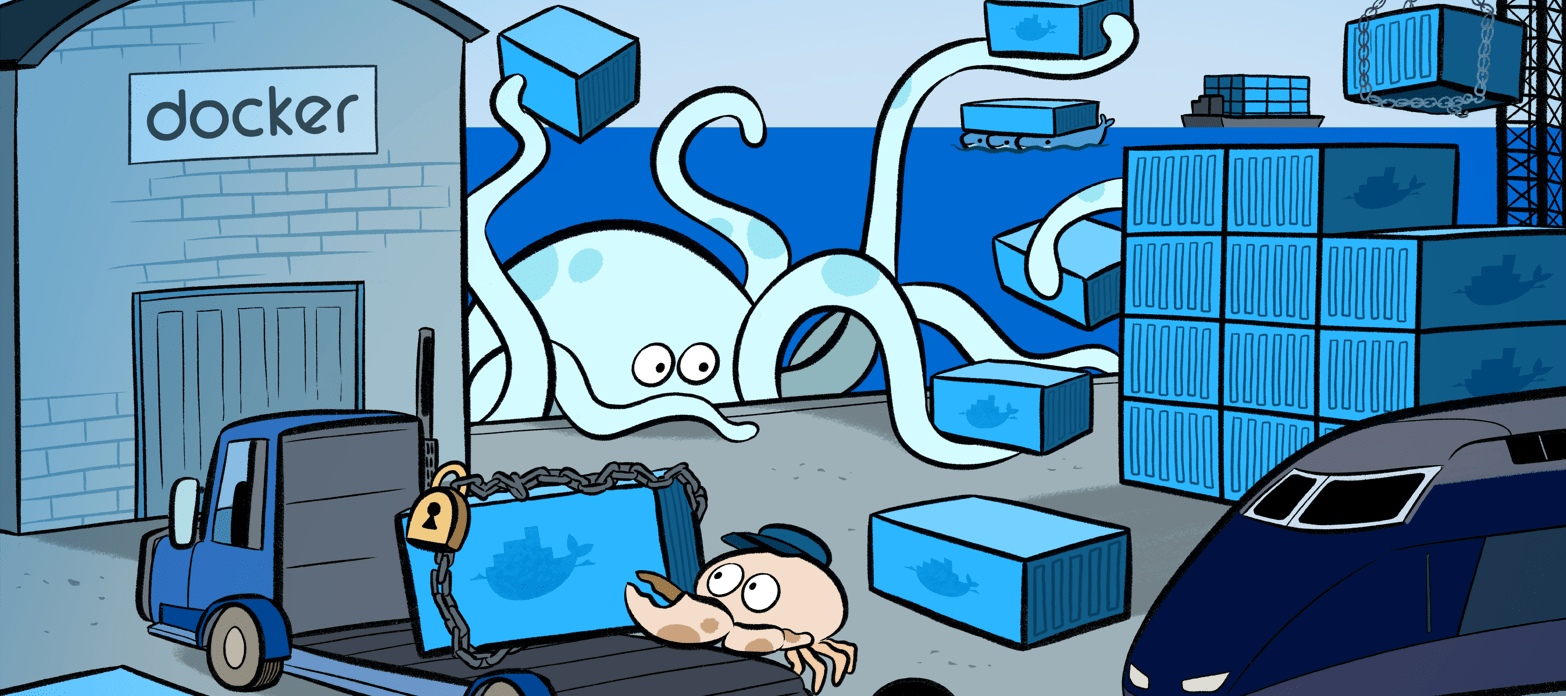
\includegraphics[width=1\textwidth]{docker.png}
\caption{<\url{https://www.docker.com}>}
\end{figure}

리눅스를 설치해서 웹서비스를 돌릴 환경을 갖추고 정기적으로 관리하는 일도, 말로 하는 것보다 훨씬 어려운 경우가 있습니다. 내가 원하는 애플리케이션이 필요로 하는 라이브러리가 빠져 있어서 추가로 설치해야 할 때도 있고, 사소하게는 버전이 안 맞아서 문제가 될 때도 있습니다. 내 로컬에 있는 리눅스에서는 잘됐는데, 정작 운영해야 할 서버에서는 뭔가 문제가 있어서 잘 실행되지 않아서, 그 문제를 해결하는 데에 많은 시간을 낭비하게 되기도 합니다.

도커는, 그 리눅스 안에 다른 가상 리눅스 환경을 여럿 만들고, 그 환경마다 각양각색의 원하는 설정을 미리 준비해서 쉽게 곧바로 실행할 수 있습니다. 필요한 오픈소스 애플리케이션이 있다면, 누군가 잘 만들어 놓은 컨테이너 이미지를 받아다가 내가 원하는 입맛으로 살짝 바꿔 실행할 수도 있고, 그대로 써도 되는 경우도 많습니다.

무엇보다 이 컨테이너를, 내 로컬 환경과 서버가 운영되는 실제 서비스 환경에서 차이 없이 그대로 쓸 수 있다는 점도 참 매력적입니다. 도커는 워낙 파격적이라 제가 설명드리는 내용이 전부이기는 어렵고요, 앞으로는, 아니 그리고 어쩌면 이미 도커로 판이 바뀌었다고 보셔도 되지 않을까 싶습니다.

어쩌면 어떤 분들은 서버용 운영체제로 리눅스가 아니라 윈도 서버를 쓰려하실 수도 있으나, 이 도커의 존재만으로도 리눅스를 써야 할 만한 충분한 이유가 되지 않을까 합니다.

\begin{itemize}
\item{Do} - 도커 기초 서적 1권을 골라 차근히 읽습니다. 당장 이해가 되지 않더라도, 일단 끝까지 읽습니다.
\end{itemize}

\section[AWS]{아마존 웹 서비스\sub{AWS, Amazon Web Services}}

예전에는, 그리고 지금도 큰 기업들은, IDC라고 인터넷 데이터 센터에 입주해서 전용 공간에서 서버를 가져다 놓고 운영합니다. 그러려면 우선 데이터 센터에 서버가 들어갈 물리적 공간과 네트워크와 전력과 항온항습 등을 위한 계약을 하고, 적절한 장비를 사서 넣어서 운영하며 관리합니다.

하지만, 이제 클라우드 환경으로 가면서, 그럴 필요가 없어졌지요. 아마존 웹 서비스 같은 플랫폼에 가입해서, 원하는 사양의 가상 머신을 원하는 순간에 필요한 시간만큼 운영할 수 있습니다. 초기에 큰 액수의 계약을 한다거나, 내게 필요한 사양의 서버를 사서 갖다 넣는다거나 하는 일은 오래전 일이 돼버렸습니다.

이미 준비된 서버들을 필요에 따라 임대해서 쓰고, 더 이상 필요 없으면 반납하면 됩니다. 내 서버를 내 자가용이라고 비유한다면, 그 이후 있었던 서버 임대 서비스가 렌터카 서비스이고, 클라우드 환경은 쏘카 같은 시스템이라고 보면 되려나요? 그보다 더 편리한 격차가 크기는 한데, 개념적으로는 크게 다르지 않을 것 같습니다. 아무튼, 지금은 서버를 산다거나 데이터센터나 호스팅 업체에 계약을 할 필요는 없고, AWS 같은 클라우드 서비스를 필요에 맞게 쓰면 됩니다.

경쟁 서비스로는 구글 클라우드 플랫폼이나 마이크로 소프트 애저가 있습니다만, AWS가 워낙에 넘사벽으로 앞서 있어서 어떨지 모르겠네요. 나중에야 상향 평준화되겠지만, 지금은 그냥 고민 없이 AWS를 쓰면 됩니다.

이 연재에서 목표로 하는 동네 웹서비스 목적으로 아주 작은 장비를 할당받아서 24시간 운영한다면, 아마도 한 달에 1\textasciitilde2만원으로도 충분하지 않을까 합니다. 다른 호스팅 업체를 이용하면 훨씬 저렴하게 운용할 수 있다고 말하는 사람들이 있을 텐데요, 고맙다 말하고 무시합니다. 커피 한 두잔 값 차이에, 불필요한 시간을 낭비하지 않아도 되니, 우리의 가장 소중한 자원인 ``시간과 노력''을 줄일 수 있다면, 충분히 지불할 만한 가격 차이입니다.

게다가, AWS의 RDS처럼 데이터베이스를 편리하게 운영해주고 백업과 복구도 대신해주는 시스템이 있어서 편리함을 넘어서서 무섭기까지 합니다. 이 정도라면 DBA 같은 직종이 덜 각광 받을 것 같고, 좀 더 지나면 저 같은 서버 개발자도 필요 없어질 것 같습니다.

다만, AWS는 워낙 방대한 서비스이기에 조금 시간을 들여 공부해야 할 필요가 있습니다. 우선 기초 서적 한 두권 골라서 여유롭게 차근히 보시고 접근하시면 좋지 않을까 합니다. 일단은 EC2, RDS, S3정도만 파악해서 쓰셔도 충분할 거예요.

\begin{itemize}
\item{Do} - AWS 기초 서적을 1권 다 읽으며 가볍게 실험해 봅니다.
\item{Don't} - 직접 서버를 운영한다거나 호스팅 업체에 입주하는 일은 하지 않습니다.
\end{itemize}

\section{마무리}

이상, 2017년에 새로 웹 개발을 시작하는 분들을 위한 하나의 이정표를 작성해 보았습니다. 시작부터 언급드렸듯이, 이게 하나의 완전한 가이드일 수는 없고요, 다만, 지나치게 흔들리거나 방황하지 말고, 시작점부터 끝점까지 하나 이어보자는 목표로 적어보았습니다. 하나하나의 주제를 학습하는 데에도 적지 않은 시간이 걸리겠지만, 다 걷고 난다면, 사실 동네 웹서비스뿐 아니라 제대로 된 개발자로 일하는 데에도 충분하지 않을까요?

이상 긴 글 다 읽어주신 분들 감사드립니다. 아마 당분간은 다른 주제로 글을 쓰겠지만, 언젠가 이 연재의 시즌2를 다시 시작할지도 모르겠네요. 그럼 즐거운 웹 개발 시작하시길 바라겠습니다!

\end{document}
